%*************************************************************************
\section{Erstellen von Editierregeln}
%*************************************************************************
\subsection{Metamodell}\label{subsec:metamodel}
Abbildung \ref{statemachine_metamodel} stellt ein Metamodell für \textit{Zustandsautomaten} (engl. \textit{statemachines}) ähnlich dem der UML dar.

\begin{figure}[H]
\centering
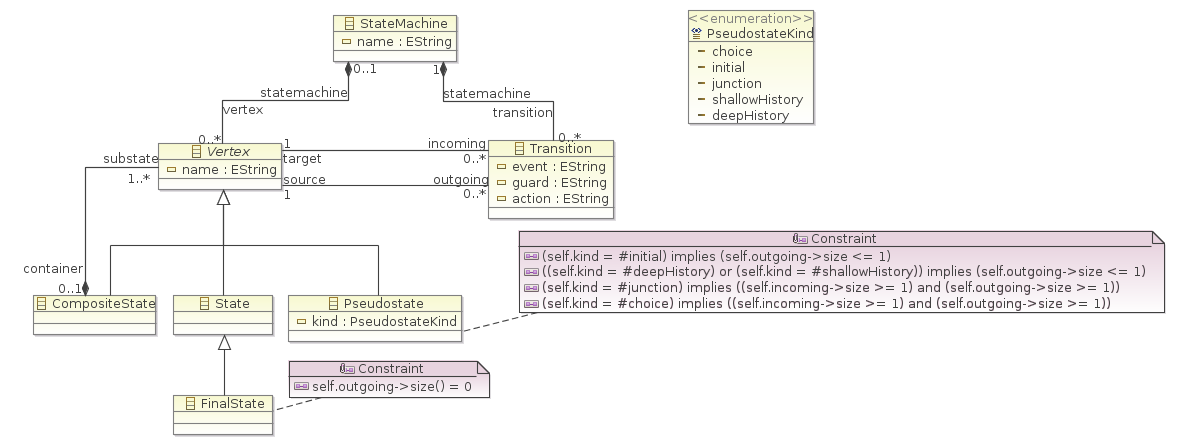
\includegraphics[width=\textwidth]{editrules/graphics/statemachine.png}
\caption{Zustandsautomat Metamodell}
\label{statemachine_metamodel}
\end{figure}

Ein \textit{Zustandsautomat} (\texttt{StateMachine}) besteht aus einer endlichen Anzahl von \textit{Zuständen} (\texttt{Vertex}) und \textit{Transitionen} (\texttt{Transition}).
Bei den Zuständen wird zwischen \textit{normalen Zuständen} (\texttt{State}), \textit{Pseudozuständen} (\texttt{Pseudostate}), \textit{Endzuständen} (\texttt{FinalState}) und \textit{zusammengesetzten Zuständen} (\texttt{CompositeState}) unterschieden.
Eine \textit{Transition} verbindet immer zwei Zustände und  kann ein \textit{Ereignis} (\texttt{Event}),  eine \textit{Bedingung} (\texttt{Guard}) und einer \textit{Aktion} (\texttt{Action}) besitzen.\\
Neben den Kardinalitäten der Referenzen sind weitere Konsistenzkriterien durch \textit{OCL-Ausdrücke} definiert. 
So darf z.B. eine Startzustand (\texttt{PseudostateKind: initial}) keine eingehende und maximal eine ausgehende Transition besitzen.\\
Im Folgendem lernen Sie ausgehend von dem vorgestellten Metamodell Editierregeln mit Hilfe von \textit{Henshin-Regeln} zu erstellen.\\

\textbf{Hinweis}: SiLift unterstützt momentan nur \textit{statisches EMF}, d.h. dass das Metamodell als \textit{Eclipse-Plugin} "'\textit{deployed}"' sein muss.

\subsection{Exkurs in EMF-Henshin}

Bei \textit{Henshin} handelt es sich um eine Transformationsprache bzw. ein Graphersetzungssystem für \textit{EMF Modelle}. 
Modelle werden als \textit{Graphen} interpretiert (man spricht hier auch von dem Arbeitsgraphen, der das Modell repräsentiert) und nach \textit{Teilgraphen} durchsucht, die vorher in einer sogenannten \textit{Transformationsregeln} definiert wurden.
Man spricht bei diesem Teilgraphen von der \textit{Left-Hand Side} (kurz \textit{LHS}) der Trans\-for\-ma\-tions\-re\-gel. 
Wird ein solcher Teilgraph gefunden wird er durch die sogenannte \textit{Right-Hand Side} (kurz \textit{RHS}) der Transformationsregel ersetzt. 
Dabei werden die Knoten und Kanten, die in der linken und nicht in der rechten Seite vorkommen gelöscht und die, die in der rechten Seite und nicht in der linken vorkommen werden erzeugt.
Knoten, die in beiden Seiten vorkommen bleiben unverändert.
Man spricht bei diesen Knoten auch vom Kontext der Transformationsregel.
Dieser Kontext kann durch sogenannte \textit{Negative Application Conditions} (kurz \textit{NACs}) weiter eingeschränkt werden.\footnote{Einführende Beispiele finden Sie unter \url{http://www.eclipse.org/henshin/examples.php}.}\\
Mehrere Regeln lassen sich in einem \textit{Modul} (engl. \textit{module}) zusammenfassen, wobei die Reihenfolge der Ausführung der Regeln durch sogenannte \textit{Units} bestimmt wird: \texttt{Independent Unit}, \texttt{Sequential Unit}, \texttt{Conditional Unit}, \texttt{Priority Unit}, \texttt{Iterated Unit} und \texttt{Loop Unit}.\\

\textbf{Hinweis}: Momentan verlangt SiLift für jede Editieroperation immer ein Transformationssystem mit genau einer \textit{mainUnit} (\texttt{Independent}, \texttt{Priority} oder \texttt{Sequential}) und einer darin enthaltenen Regel. Eine Ausnahme bilden geschachtelte Regeln, in der eine \textit{Kernel-Regel} und eine beliebige Menge von \textit{Multi-Regeln} definiert werden.


Henshin stellt zum Entwickeln von Transformationsystemen zwei Editoren zur Verfügung:

\begin{enumerate}

\item \textbf{Henshin Transformation Model Editor}: 
Ein baumbasierter Editor mit ent\-sprech\-en\-der linken und rechten Seite der Transformationsregeln (vgl. Abb.\ref{silift-editrule_createStateInStateMachine}: links).

\item \textbf{Henshin Diagram Editor}: 
Ein graphenbasierter Editor mit den \textit{"'Stereotypen"'} \texttt{create}, \texttt{delete}, \texttt{preserve}, \texttt{require} und \texttt{forbid} zum markieren entsprechender Operationen (vgl. Abb. \ref{silift-editrule_createStateInStateMachine}: rechts).
Knoten und Kanten die mit \texttt{delete} markiert sind, kommen nur in der \textit{LHS} vor, wohingegen Knoten und Kanten, die mit \texttt{create} markiert sind nur in der \textit{RHS} vorkommen.
Knoten, die auf beiden Seiten vorkommen werden als \texttt{preserve} markiert.
Mit \texttt{require} und \texttt{forbid} lassen sich Teilgraphen erzeugen, die in einem Kontext auftreten müssen bzw. nicht auftreten dürfen.
\end{enumerate}

\subsection{Atomare Editierregeln}

Wie bereits erwähnt umfassen die atomaren Regeln das Erzeugen, Löschen, Verschieben von Elementen und das Ändern von Attributwerten.
Um eine Editierregel zu erstellen legen Sie ein neues Projekt an und wählen Sie \texttt{File} $\triangleright$ \texttt{New} $\triangleright$ \texttt{Other...} und hier \texttt{Henshin Model} aus. 
Klicken Sie auf \texttt{Next} (vgl. Abb. \ref{henshin-create_henshin_model_page01}).\\
%Im nächsten Dialog wird nach einem Dateinamen gefragt. 


\begin{figure}[H]
\centering
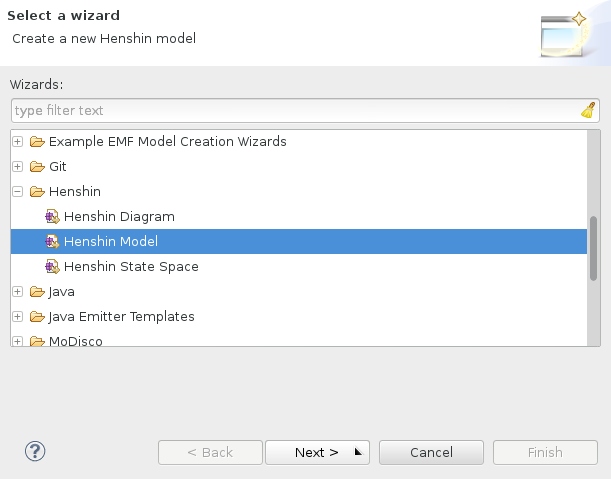
\includegraphics[width=0.6\textwidth]{editrules/graphics/henshin-create_henshin_model_page01.png}
\caption{Erstellen eines neuen Transformationsmodells: Page 1}
\label{henshin-create_henshin_model_page01}
\end{figure}

Die Datei kann einen beliebigen Namen bekommen, jedoch muss sie auf \texttt{\_execute.henshin} enden.
Da der Name der Regel eindeutig sein muss ist es zu empfehlen die Datei nach ihrer späteren Regel zu benennen. Somit behalten Sie den Überblick.
Die folgende Regel soll einen Zustand in einen vorhanden Zustandsautomaten einfügen. Hier würde sich bspw. der Name \texttt{Create\_StateInStateMachine\_execute.henshin} anbieten (vgl. Abb.\ref{henshin-create_henshin_model_page02}).
Wählen sie den Zielordner und geben Sie den Dateinamen ein.
Klicken Sie auf \texttt{Next}.

\begin{figure}[H]
\centering
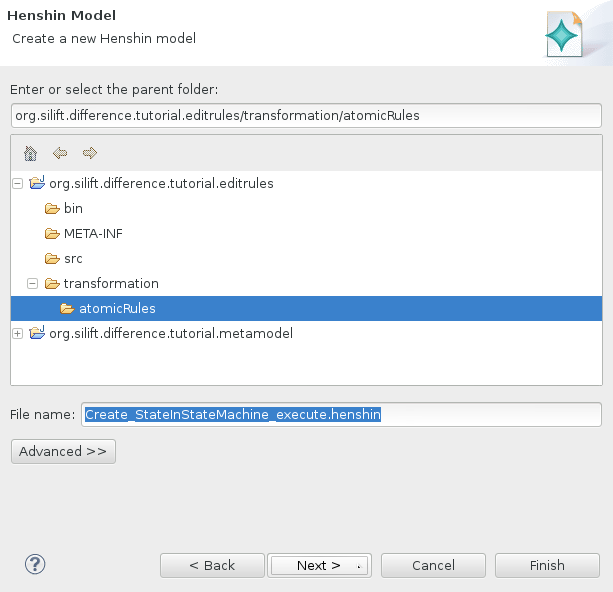
\includegraphics[width=0.6\textwidth]{editrules/graphics/henshin-create_henshin_model_page02.png}
\caption{Erstellen eines neuen Transformationsmodells: Page 2}
\label{henshin-create_henshin_model_page02}
\end{figure}

Als letztes müssen Sie noch Ihr Metamodel aus der Registry (\texttt{Add From Registry}) laden (vgl. Abb. \ref{henshin-create_henshin_model_page03}).

\begin{figure}[H]
\centering
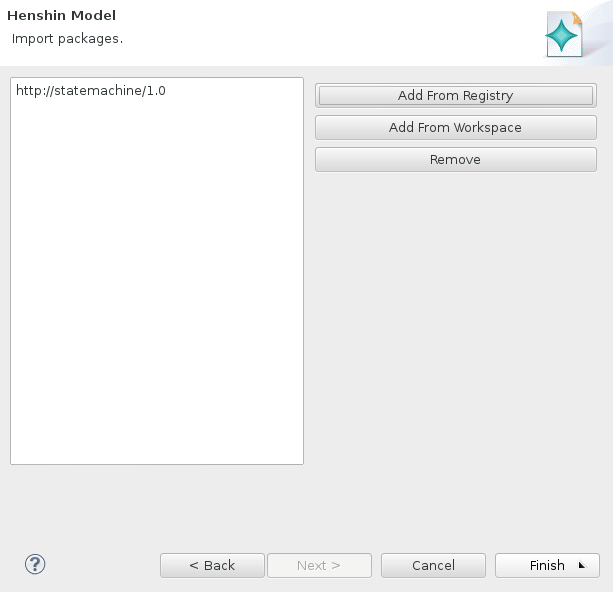
\includegraphics[width=0.6\textwidth]{editrules/graphics/henshin-create_henshin_model_page03.png}
\caption{Erstellen eines neuen Transformationsmodells: Page 3}
\label{henshin-create_henshin_model_page03}
\end{figure}

Um neben dem baumbasierten auch den graphenbasierten Editor nutzen zu können muss zusätzlich noch ein \textit{Henshin-Diagramm} erzeugt werden.
Klicken Sie hierzu mit der rechten Maustaste auf die \texttt{CREATE\_StateInStateMachine\_execute.henshin}, wählen Sie \texttt{Henshin} $\triangleright$ \texttt{Initialize Diagram File} aus und folgen Sie dem Assistenten (vgl. Abb. \ref{henshin-initialize_henshin_diagram}).

\begin{figure}[H]
\centering
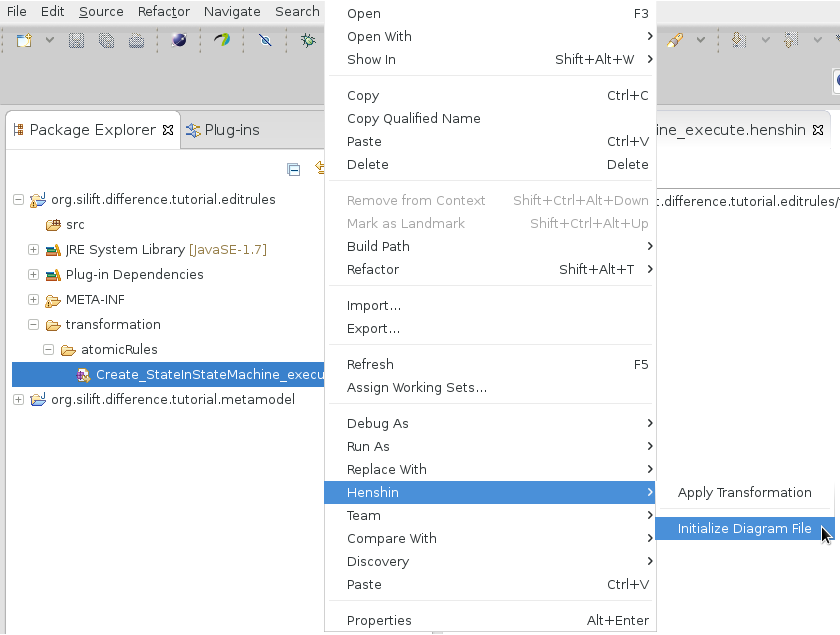
\includegraphics[width=0.5\textwidth]{editrules/graphics/henshin-initialize_henshin_diagram.png}
\caption{Erstellen eines Henshin Diagramms}
\label{henshin-initialize_henshin_diagram}
\end{figure}

\subsubsection*{Create-Regeln}

Erstellen Sie eine Regel, indem sie aus der Palette das \textit{Rule-Werkzeug} auswählen und danach auf die Arbeitsfläche klicken. Geben Sie der Regel den Namen \texttt{create""State""In""State""Machine}.
Einer Regel können ähnlich einer Funktion oder Methode Parameter übergeben werden (vgl. Abb. \ref{silift-editrule_createStateInStateMachine}).
Dabei lässt sich zwischen \textit{Object-} und \textit{Value-Parametern} unterscheiden:

\begin{itemize}

\item \textbf{Object-Parameter}: 
Durch Objekt-Parameter können Objekte an die Regel über\-ge\-ben werden, um diese gezielt aus dem Arbeitsgraphen zu löschen, in dem Arbeitsgraphen zu erzeugen oder zu verändern.
Des Weiteren können dadurch Kontextobjekte eindeutig bestimmt werden. 
Sofern der Objekt-Parameter ein zu löschenden Knoten identifiziert handelt es sich um einen \textit{in}-Parameter.
Repräsentiert der Parameter hingegen ein zu erzeugendes Objekt handelt es sich um einen \textit{out}-Parameter (vgl. Seite \pageref{in/out_parameter}).

\item \textbf{Value-Parameter}: Mit Hilfe von Value-Parametern können (Attribut-) Werte (z.B. Zeichenketten, Zahlen etc.) übergeben, verglichen und neu berechnet werden.
\end{itemize}

Für das Erzeugen eines neuen Zustands wird ein Parameter (\texttt{Selected}) benötigt, der den Zustandsautomaten, in den ein neuer Zustand eingefügt werden soll, identifiziert, sowie ein Parameter der den erzeugten Zustand zurück gibt (\texttt{New}).\\
Danach müssen mit Hilfe des \textit{Node-Werkzeugs} die beiden Knoten (\texttt{Nodes}) vom Typ \texttt{StateMachine} und \texttt{State} erstellt und der entsprechende Parameter voran gestellt werden (vgl. Abb. \ref{silift-editrule_createStateInStateMachine}).
Wählen Sie aus der Palette das \textit{Edge-Werkzeug} und verbinden Sie die beiden Knoten miteinander, um die Kanten zwischen den gerade erstellten Knoten zu ziehen.
Sofern nicht bereits der gewünschte Typ der Kanten erzeugt wurde, kann dieser unter den \textit{Properties} angepasst werden. 
Selektieren Sie dazu die entsprechende Kante mit der rechten Maustaste und wählen Sie \texttt{Show Properties View}.\\
%Bei den Kanten \texttt{incoming} und \texttt{outgoing} aus dem Metamodell (vgl. Abb. \ref{statemachine_metamodel}) handelt es sich um abgeleitete (engl. \textit{derived}) Referenzen. Diese dürfen nicht durch Editierregeln erstellt werden. 

\textbf{Hinweis}: Abgeleitete (engl. \textit{derived}) Referenzen dürfen nicht durch Editierregeln erstellt werden.


\begin{figure}[H]
\centering
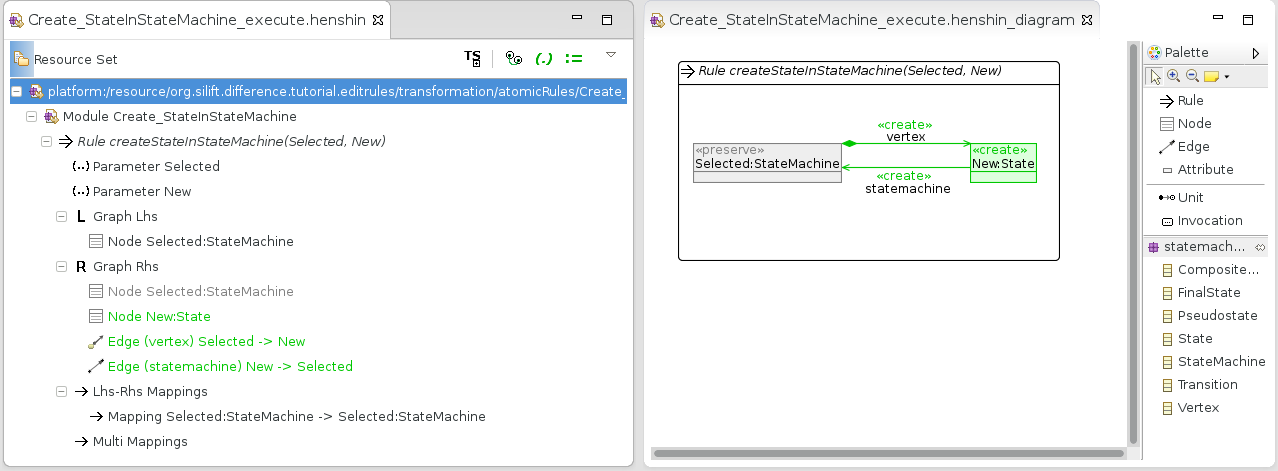
\includegraphics[width=0.8\textwidth]{editrules/graphics/silift-editrule_createStateInStateMachine.png}
\caption{Editierregel: createStateInStateMachine}
\label{silift-editrule_createStateInStateMachine}
\end{figure}

Wie bereits erwähnt, verlangt SiLift für jede Editieroperation immer ein Modul mit genau einer Unit und (mit Ausnahme geschachtelter Regeln) einer darin enthaltenen Regel.
Diese Unit muss per Konvention den Namen \textit{mainUnit} tragen.\\
Zwar lassen sich die Units ebenfalls im graphenbasierten Editor erstellen, dennoch ist in unserem Fall der baumbisierte Editor zu bevorzugen.\\
Wechseln Sie in den baumbasierten Editor, indem sie die \texttt{*\_execute.henshin} öffnen.
Im Gegensatz zur graphischen Repräsentation der Regel, lassen sich im baumbasierten Editor die linke und rechte Seite der Transformationsregel genau unterscheiden.
Beim Anwenden einer Regel wird der Arbeitsgraph auf das Vorkommen des Teilgraphen der LHS untersucht. In unserem Beispiel also auf den Teilgraphen, der nur  einen Knoten vom Typ \texttt{StateMachine} enthält.
Durch einen Objekt-Parameter sagen wir zusätzlich um welchen Knoten vom Typ \texttt{StateMachine} es sich genau handeln muss.
Existiert ein solcher Teilgraph, so wird dieser durch den Graphen der RHS ersetzt.
In diesem Fall also einer \texttt{StateMachine}, einem \texttt{State} und den beiden Referenzen \texttt{statemachine} und \texttt{state}.
Zu beachten ist, dass es sich bei dem \texttt{StateMachine}-Knoten um einen "'\textit{preserve}"'-Anteil der Regel handelt, also einem Knoten der eigentlich nicht verändert wird. 
Dazu muss dieser Knoten auf beiden Seiten der Regel vorkommen und ein sogenanntes \textit{Mapping} zwischen diesen existieren (vgl. Abb. \ref{silift-editrule_createStateInStateMachine}: links).\\
Zum Erstellen der mainUnit klicken Sie mit der rechten Maustaste auf \texttt{Module} und wählen \texttt{New Child} $\triangleright$ \texttt{PriorityUnit} (vgl. Abb \ref{silift-editrule_create_priority_unit}).

\begin{figure}[H]
\centering
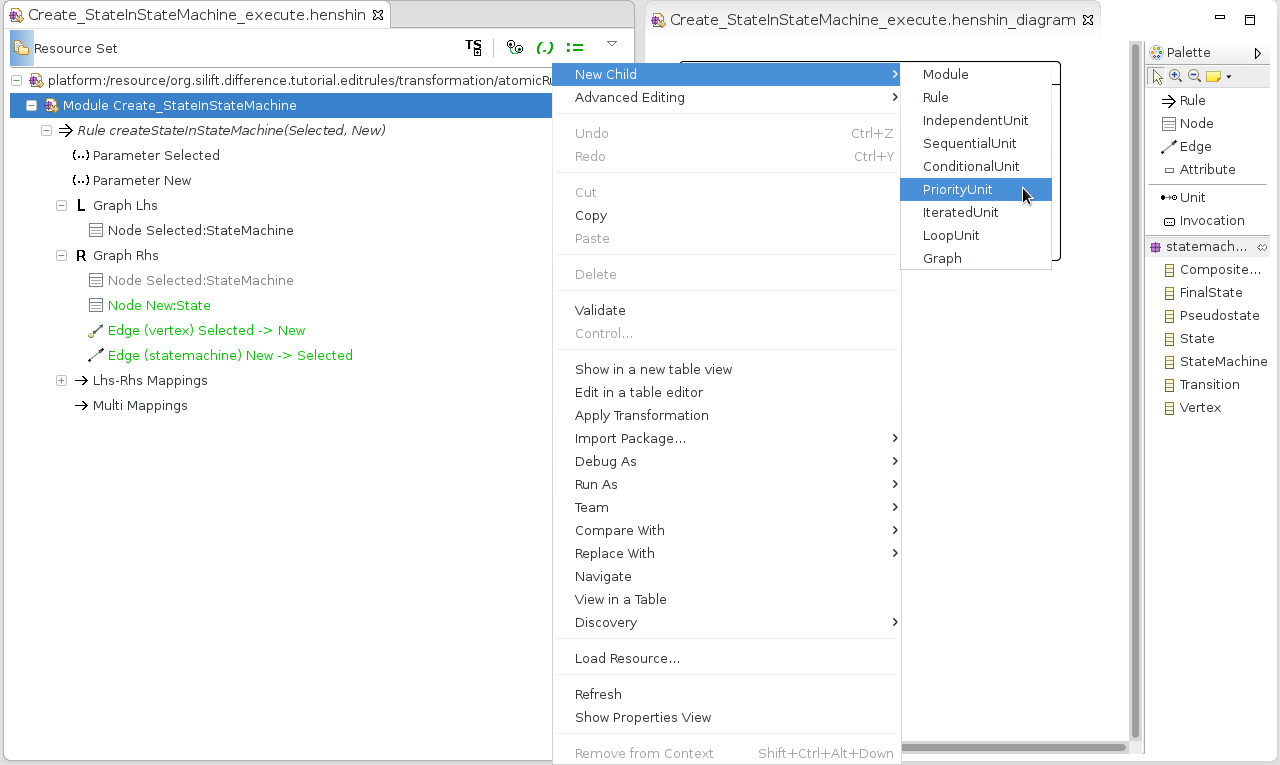
\includegraphics[width=0.8\textwidth]{editrules/graphics/silift-editrule_create_priority_unit.png}
\caption{Editierregel: Erstellen einer \textit{Priority Unit}}
\label{silift-editrule_create_priority_unit}
\end{figure}

Nennen Sie diese in "'\textit{mainUnit}"' um und kopieren Sie die eigentliche Regel per \textit{Drag and Drop} in die Unit hinein.\\
Zusätzlich muss die Unit die gleiche Anzahl an Parametern besitzen, wie die Regel. 
Selektieren Sie dazu die \textit{Priority Unit} mit der rechten Maustaste und wählen Sie \texttt{New Child} $\triangleright$ \texttt{Parameter} (vgl. Abb. \ref{silift-editrule_unit_create_parameter}). 
Dabei dürfen die Namen der Parameter durchaus von denen in der Regel abweichen.\\

\textbf{Hinweis}: In Ausnahmefällen kann eine Unit auch weniger Parameter definieren als die beinhaltete Regel. So z.B., wenn die Regel intern Variablen benötigt (z.B. bei der Berechnung von Attributwerten). Derartige interne Variablen werden in Henshin-Regeln auch als Parameter deklariert und sind von Übergabeparametern nicht zu unterscheiden. Die Parameter der Unit repräsentieren letztlich aber die extern sichtbaren Parameter der Editieroperation, also die Signatur der Editieroperation.

\textbf{WICHTIG}: Es muss immer ein \textit{in}-Parameter mit dem Namen \texttt{selectedEObject} existieren, der einen vorhanden Knoten hinein gibt, der zum Kontext der Editierregel gehört.


\begin{figure}[H]
\centering
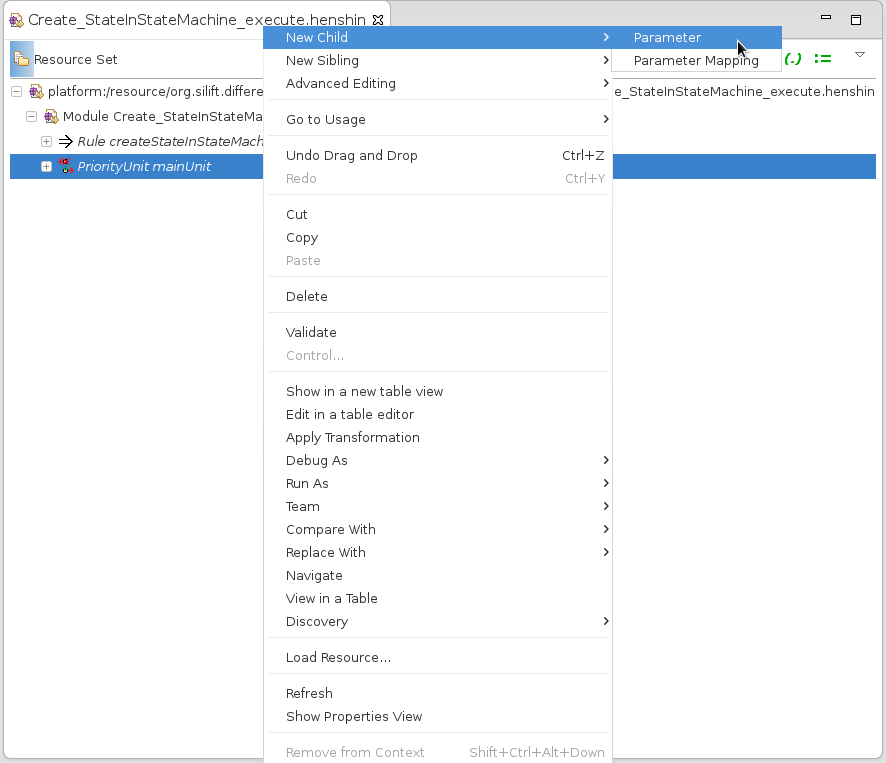
\includegraphics[width=0.6\textwidth]{editrules/graphics/silift-editrule_unit_create_parameter.png}
\caption{Editierregel: Erstellen von Parametern}
\label{silift-editrule_unit_create_parameter}
\end{figure}

Nachdem Sie die Parameter erstellt haben müssen diese nun auf die entsprechenden Parameter der Regel "'\textit{gemappt}"' werden.
Durch das \textit{Mapping} wird die Richtung der Parameter (\texttt{in}/\texttt{out}) festgelegt.
Klicken Sie wieder mit der rechten Maustaste auf die \textit{Priority Unit} und wählen Sie diesmal \texttt{New Child} $\triangleright$ \texttt{Parameter Mapping}.\\
Jedes \textit{Parameter-Mapping} besteht aus einem \texttt{Source}- und \texttt{Target}-Parameter, welche unter der \textit{Properties-View} gesetzt werden können.\\

\label{in/out_parameter}
Wird ein Parameter der \textit{Unit} auf einen Parameter der \textit{Rule} gemappt, so handelt es sich um einen \textit{in-Parameter} der aus dem aktuellen Arbeitsgraphen ein Objekt bzw. Knoten an die Regel übergibt (vgl. Abb. \ref{silift-editrule_parametermapping_in}). 
Für \texttt{selectedEObject} ist das immer der Fall. 
Das gleiche gilt für Objekte die gelöscht werden sollen.

\begin{figure}[H]
\centering
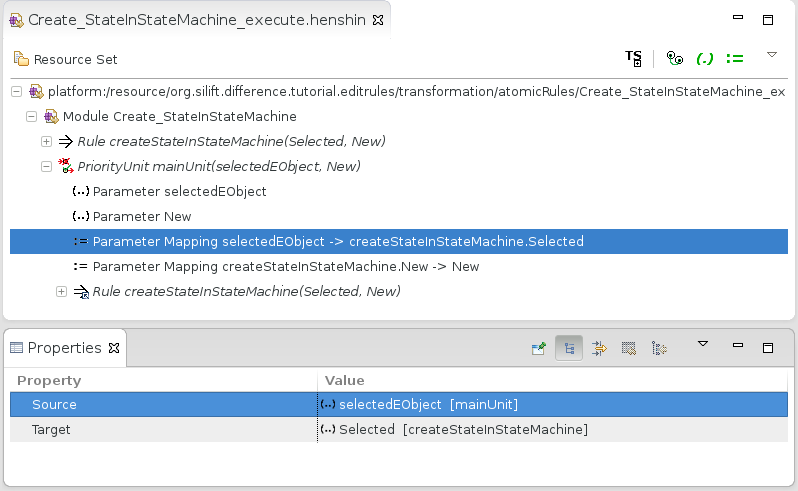
\includegraphics[width=0.6\textwidth]{editrules/graphics/silift-editrule_parametermapping_in.png}
\caption{Editierregel: \textit{in-Parameter}}
\label{silift-editrule_parametermapping_in}
\end{figure}

Objekte, welche durch die \textit{Rule} erzeugt werden, müssen durch \textit{out-Parameter}, über die \textit{Unit} zurück an den Arbeitsgraphen gegeben werden.
D.h. der entsprechende Parameter der \textit{Rule} muss auf einen Parameter der \textit{Unit} gemappt werden (vgl. \ref{silift-editrule_parametermapping_out}).
 
\begin{figure}[H]
\centering
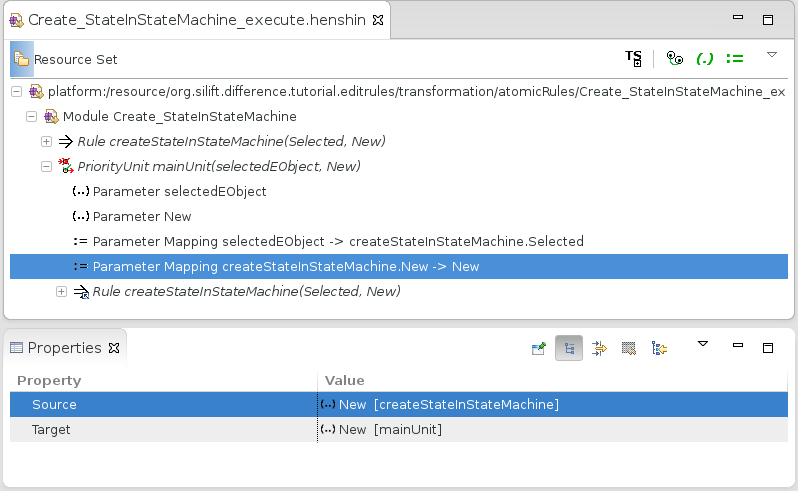
\includegraphics[width=0.6\textwidth]{editrules/graphics/silift-editrule_parametermapping_out.png}
\caption{Editierregel: \textit{out-Parameter}}
\label{silift-editrule_parametermapping_out}
\end{figure}

Damit ist die Regel \texttt{createStateInStateMachine} fertig.


\subsubsection*{Delete-Regeln}

Im vorherigem Abschnitt haben Sie gelernt, worauf Sie beim Erstellen einer \textit{Create-Regel} achten müssen.
Neben dem Hinzufügen einzelner Modellelemente, benötigt man jedoch auch Regeln, um Elemente zu verschieben oder aus dem Modell zu entfernen.\\
Erstellen Sie analog zum vorherigem Abschnitt ein neues Henshin-Modell mit dem Namen \texttt{DELETE\_StateInStateMachine\_execute.henshin} und dem entsprechenden Diagramm.
Ersetzen Sie den \textit{"'Stereotypen"'} \texttt{create} durch \texttt{delete} (vgl. Abb \ref{silift-editrule_deleteStateInStateMachine}).

\begin{figure}[H]
\centering
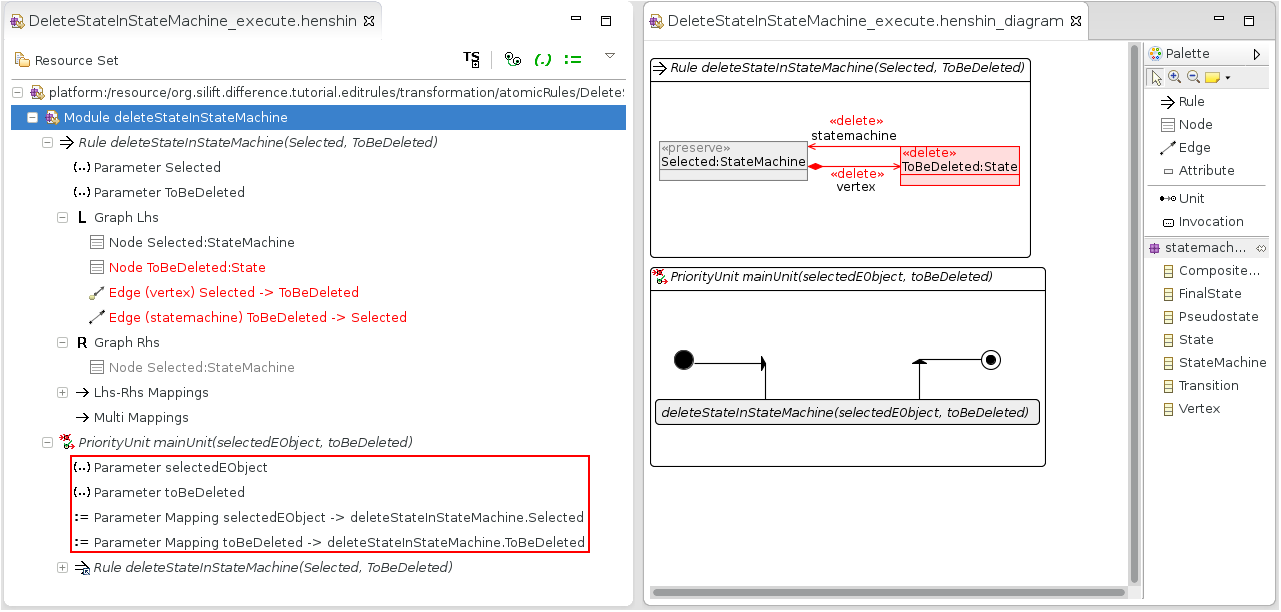
\includegraphics[width=0.8\textwidth]{editrules/graphics/silift-editrule_delete_stateInStateMachine.png}
\caption{Editierregel: \texttt{deleteStateInStateMachine}}
\label{silift-editrule_deleteStateInStateMachine}
\end{figure}

Zu beachten ist, dass dieser Regel anstatt einem, zwei Objekte übergeben wird. 
Des Weiteren gibt die Regel auch kein Objekt zurück. 
Dem entsprechend muss das Parameter Mapping angepasst werden (vgl. Abb. \ref{silift-editrule_deleteStateInStateMachine}).\\
Ein weiterer wichtiger Punkt beim Löschen von Elementen sind sogenannte \textit{hängende Referenzen} (engl. \textit{dangling edges}).\\
Abbildung \ref{statemachine_garagedoor} beschreibt die Funktionsweise eines Garagentors in Form eines Zustandsautomaten. 
Initial ist der Zustandsautomat im Zustand \texttt{geschlossen}. 
Bei Tastendruck wird der Zustand \texttt{öffnend} eingenommen usw.

\begin{figure}[H]
\centering
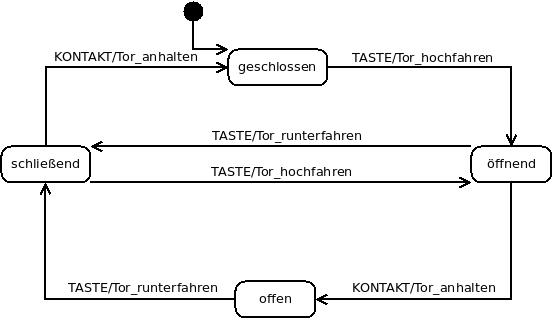
\includegraphics[width=0.5\textwidth]{editrules/graphics/statemachine-garagedoor.jpg}
\caption{Zustandsautomat: Garagentor}
\label{statemachine_garagedoor}
\end{figure}

Die interne Repräsentation des Modells, mit der Henshin arbeitet, ist in Abbildung \ref{henshin_workinggraph_garagedoor} zu sehen. 
Um die Übersicht zu behalten wurden, mit Ausnahme der umrandeten Elemente ,einige Referenzen ausgelassen.  

\begin{figure}[H]
\centering
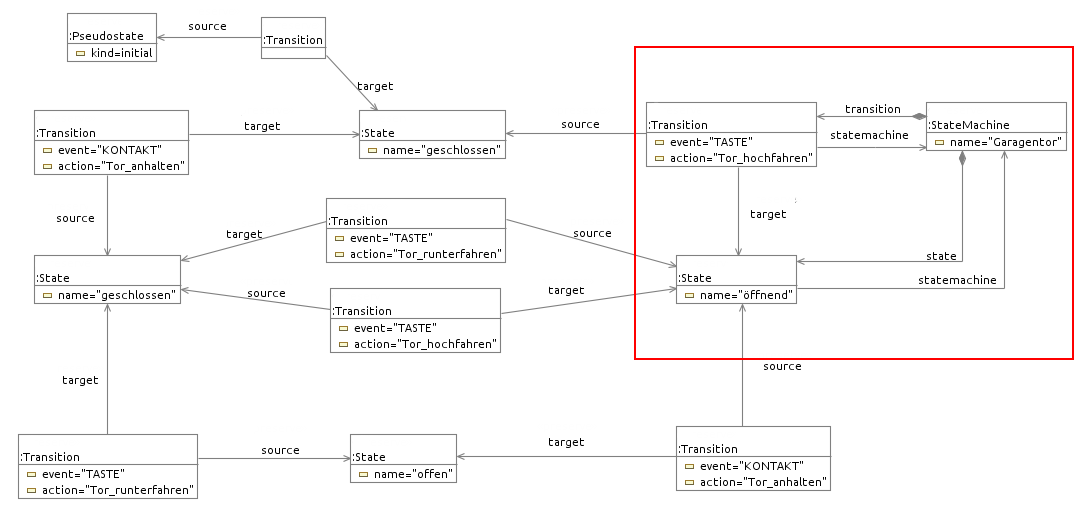
\includegraphics[width=0.8\textwidth]{editrules/graphics/henshin-workinggraph_garagedoor.png}
\caption{Arbeitsgraph}
\label{henshin_workinggraph_garagedoor}
\end{figure}

Beim Anwenden der Regel \texttt{deleteSateInStateMachine}, um z.B. den Zustand \texttt{öffnend} zu löschen, würden hängende Referenzen und somit ein inkonsistentes Modell entstehen. Die Regel löscht nur die Referenzen zwischen \textit{StateMachine} und \textit{State}, alle anderen bleiben bestehen (vgl. Abb. \ref{henshin_workinggraph_garagedoor_danglingEdges}). 

\begin{figure}[H]
\centering
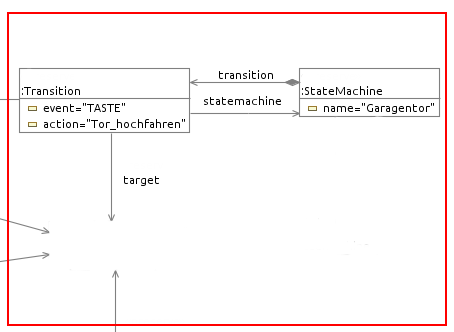
\includegraphics[width=0.5\textwidth]{editrules/graphics/henshin-workinggraph_garagedoor_danglingEdges.png}
\caption{hängende Referenzen}
\label{henshin_workinggraph_garagedoor_danglingEdges}
\end{figure}

Um in so einem Fall das Anwenden einer Regel zu verhindern, muss für die entsprechende Regel die Option \texttt{Check Dangling} auf \texttt{true} gesetzt sein (vgl. \ref{silift-silift-editrule_delete_stateInStateMachine_checkDangling}).\\

\textbf{Hinweis}: Die Option \texttt{Check Dangling} ist per \textit{default} auf \texttt{true} gesetzt und sollte bei der Verwendung von \textit{SiLift} auch nicht geändert werden.


\begin{figure}[H]
\centering
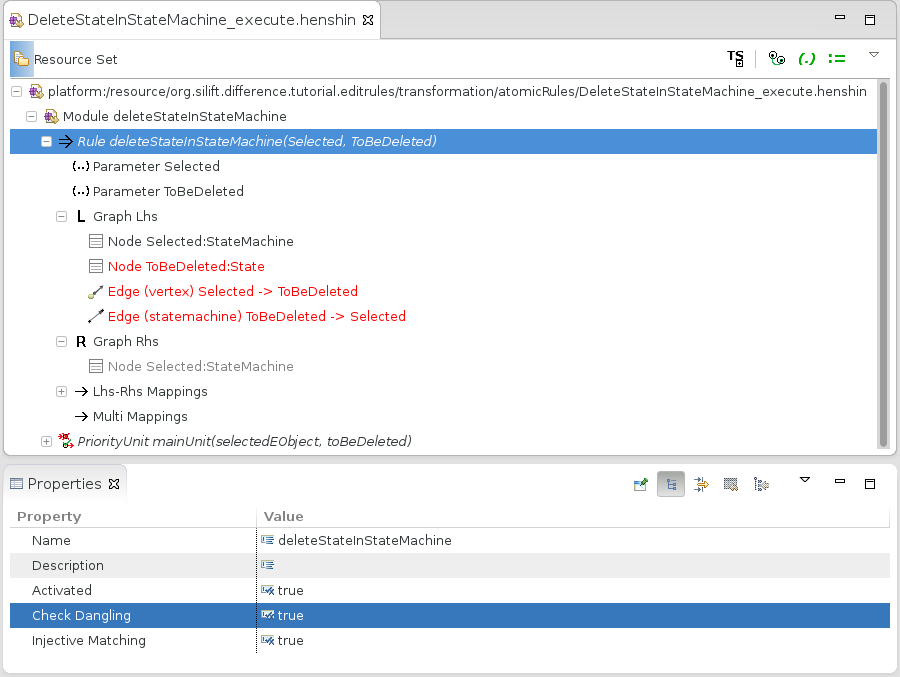
\includegraphics[width=0.6\textwidth]{editrules/graphics/silift-editrule_delete_stateInStateMachine_checkDangling.png}
\caption{hängende Referenzen}
\label{silift-silift-editrule_delete_stateInStateMachine_checkDangling}
\end{figure}


\subsubsection*{Negative Application Conditions}

Abbildung \ref{silift-editrule_create_transitionFromInitialToState} zeigt eine Editierregel, die eine neue Transition von einem Startzustand zu einem normalen Zustand erzeugt.

\begin{figure}[H]
\centering
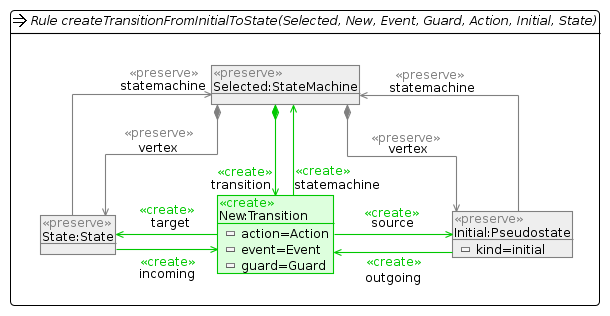
\includegraphics[width=0.6\textwidth]{editrules/graphics/silift-editrule_create_transitionFromInitialToState.png}
\caption{Editierregel: \texttt{createTransitionFromInitialToState}}
\label{silift-editrule_create_transitionFromInitialToState}
\end{figure}

Betrachtet man jetzt nochmal das Metamodell  auf Seite \pageref{subsec:metamodel}, so darf ein \textit{Startzustand} maxi\-mal eine ausgehende Transition besitzen.
Solche Bedingungen können mit \textit{NACs} umgesetzt werden.
Dazu modelliert man den unerwünschten Fall als Teilgraph und markiert diesen mit dem \textit{"'Stereotyp"'} \texttt{forbid} (vgl. Abb. \ref{silift-editrule_create_transitionFromInitialToState_with_forbid}).

\begin{figure}[H]
\centering
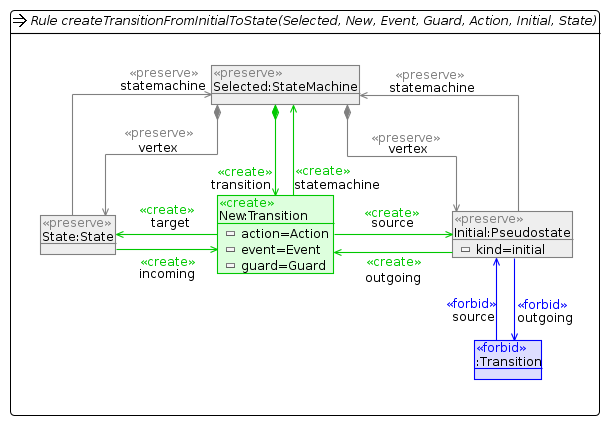
\includegraphics[width=0.6\textwidth]{editrules/graphics/silift-editrule_create_transitionFromInitialToState_with_forbid.png}
\caption{Editierregel: \texttt{createTransitionFromInitialToState} mit \textit{NAC}}
\label{silift-editrule_create_transitionFromInitialToState_with_forbid}
\end{figure}

Dieser erzeugt in der \textit{LHS} eine \texttt{Application Condition}, welche negiert wird.
Die Condition besitzt ein Graph-Objekt, welches den unerwünschten Teilgraphen modelliert.\\
In unserem Fall besteht der Teilgraph aus vier Knoten und sechs Kanten.
Zusätzlich wird noch ein Mapping der Knoten \texttt{Initial:Pseudostate}, \texttt{Selected:StateMachine} und \texttt{State:State} aus der LHS auf den NAC-Graphen benötigt (vgl. Abb. \ref{silift-editrule_create_transitionFromInitialToState_with_forbid}).


\begin{figure}[H]
\centering
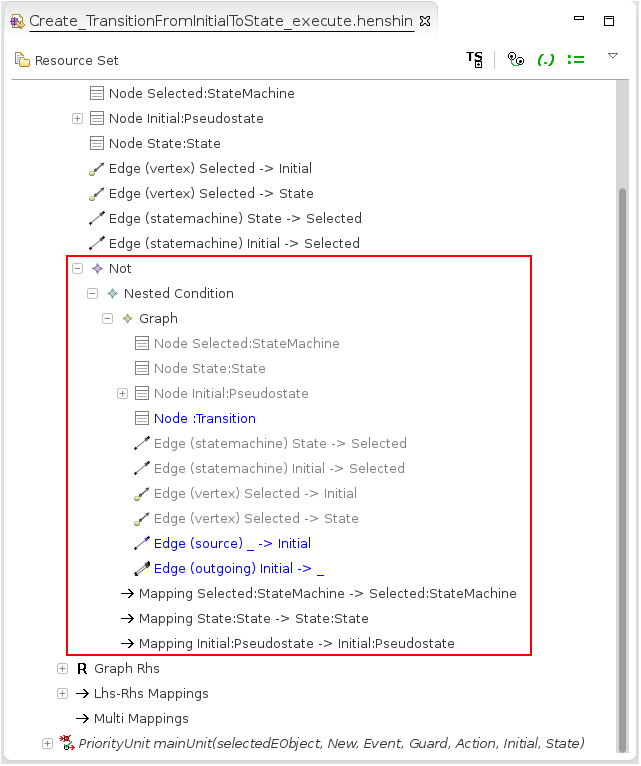
\includegraphics[width=0.5\textwidth]{editrules/graphics/silift-editrule_create_transitionFromInitialToState_with_forbid_treeView.png}
\caption{Editierregel: \texttt{createTransitionFromInitialToState} mit \textit{NAC}}
\label{silift-editrule_create_transitionFromInitialToState_with_forbid_treeView}
\end{figure}

\textbf{Hinweis}: In Henshin lassen sich \textit{NACs} beliebig schachteln und durch boolsche Operatoren wie \texttt{AND} und \texttt{OR} verknüpfen. \textit{SiLift} unterstützt in der aktuellen Version nur die Konjunktion von Anwendungsbedingungen.

